
\newpage

\index{scripting}

\noindent
Here is a simple example that draws the graph of $y=mx+b$.

\medskip
{\tt y=m*x+b}

{\tt m=1/2}

{\tt b=-3}

{\tt draw(y)}

\medskip
\noindent
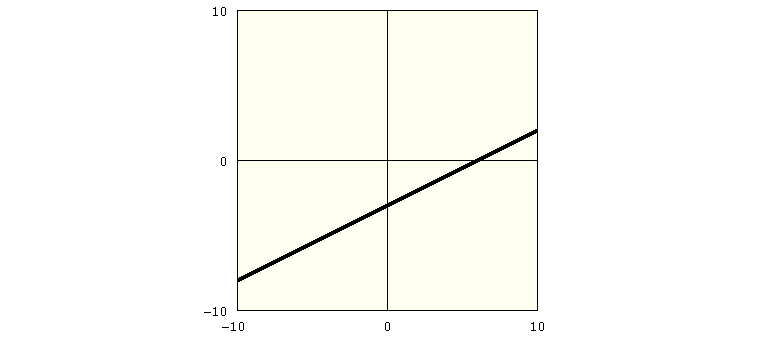
\includegraphics[scale=0.4]{1.png}

\newpage

\noindent
Now suppose that we want to draw the graph
with a different $m$.
We could type in everything all over again, but it would be easier
in the long run to write a script.
Then we can go back and quickly change $m$ and $b$ as many times as we want.

\medskip
\noindent
To prepare a script, click on the Edit Script button.
Then enter the script commands, one per line.

\medskip
{\tt y=m*x+b}

{\tt m=1/2}

{\tt b=-3}

{\tt draw(y)}

\medskip
\noindent
Next, click on the Run Script button to see the graph.

\medskip
\noindent
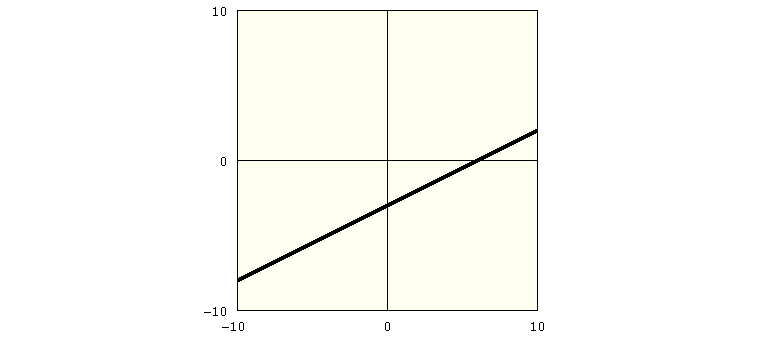
\includegraphics[scale=0.4]{1.png}

\medskip
\noindent
Eigenmath runs a script by stepping through it line by line.
Each line is evaluated just like a regular command.
This continues until the end of the script is reached.
After the script runs, you can click Edit Script and go back and change something.

\medskip
\noindent
By the way, Eigenmath automatically does a clear before
running a script.

\newpage

\noindent
Sometimes it is desirable to have a script print a few comments when it runs.
This can be accomplished by placing the desired text in quotes
on a single line.
For example, the script

\medskip
\verb$"Here is the value of pi."$

\verb$float(pi)$

\medskip
\noindent
displays the following when run.

\medskip
\verb$Here is the value of pi.$

$$3.14159$$

